\documentclass[a4paper,11pt]{report}
\usepackage[T1]{fontenc}
\usepackage[utf8]{inputenc}
\usepackage{lmodern}
\usepackage{graphicx}
\usepackage{amsmath}
\usepackage{amssymb}
\usepackage{algpseudocode}
\title{Hardware RSA Accelerator}
\author{Group 3: Ariel Anders, Timur Balbekov, Neil Forrester}


\begin{document}

\maketitle
\tableofcontents

\begin{abstract}
%Project Objective Describe the goal of the project. What problem are you trying to solve? How is the FPGA involved in the solution of that problem? Include relevant specific details such as the target frame rate, bit rate, frame dimensions, or message sizes.
Our project is implementing the RSA cryptographic algorithm in Bluespec.
The benefits of doing this in hardware are higher performance, reduced power usage and size, and cost.
Having reusable IP that implements RSA would allow a device manufacturer to either reduce their
power footprint, or skip inclusion of a processor in a device that otherwise would not need one.  

More specifically, our objective is to implement the encryption and decryption protocols in RSA for 1024 bit messages on the XUPV5 Bluespec ...speed.  (include some speed stuff here)
\end{abstract}
%%%
\chapter{Background}
CITE WIKIPEDIA!!
Assume the readers of your final report are not intimately familiar with your project
domain. Provide enough high level background about the domain or algorithms involved for
the reader to get an idea of the scope of the project and understand significant design choices
described later in the document.
Include the benefits of using an FPGA for this application.

RSA is an encryption protocol that involves a public and private key.  As indignant of its name, the public key is known to everyone and is used to encrypt messages, which are called "ciphertext".  The ciphertext can then be decrypted using the private key.  Our implementation assumes the public and private keys are generated prior to encryption through with the FPGA.    
\section{RSA Algorithm}
\subsection{Definition of Variables for the RSA Algorithm}
\begin{description}
\item[Public Key ($n$, $e$)] A public key consists of the modulus $n$ and encryption exponent $e$
\item[Private Key ($n$, $d$)]A  private key consists of the same modulus $n$ and the private decryption exponent $d$
\item[Message ($m$)] The plain text message converted into an integer $m$, such that $0 \leq m \leq n$ 
\item[Ciphertext ($c$)]  The plain text message encrypted using the public key
\end{description}
\subsection{Encryption}
The ciphertext is generated by encrypting the plain text message using the public key:
\begin{equation}
  c \equiv m^e\ (mod\ n)
\end{equation}
\subsection{Decryption}
The plaintext message is generated by decrypting the ciphertext message using the private key:
\begin{equation}
  m \equiv c^d\ (mod\ n)
\end{equation}
%%%
\section{RSA Algorithm for Hardware Implementation}
Using a naive approach to implement this algorithm would clearly run quickly out of space.  Instead, we have selected two algorithms that blablabla good space yada yada yada
Copied algorithms over... still needs to be cleaned up
\subsection{Modular Exponentiation}
This module will employ the Right-to-left binary algorithm, which we believe is a good compromise between speed, memory usage, and complexity.
The goal of the algorithm is to calculate $b^e \bmod m$ for very large values of $b$, $e$, and $m$.
If the bits of $e$ are $e_1, e_2 \dots e_n$:
\begin{equation}
e = \sum_{i = 0}^{n} e_i 2^i
\end{equation}
then:
\begin{equation}
b^e = \prod_{i = 0}^{n} e_i b^{(2^i)}
\end{equation}
and since:
\begin{equation}
a * b \bmod m = (a \bmod m) * (b \bmod m) \bmod m
\end{equation}
then every intermediate result can be taken modulo $m$ to keep the size of intermediate results manageable.
Therefore, the following algorithm will compute $b^e \bmod m$ in a reasonable amount of time and memory:
\begin{algorithmic}
\State $b$, $e$, and $m$ are the inputs to the algorithm.
\State $c \gets 1$
\While{$e > 0$}
	\If{$e \bmod 2 = 1$}
		\State $c \gets c * b \bmod m$
	\EndIf
	\State $b \gets b * b \bmod m$
	\State $e \gets \lfloor e / 2 \rfloor$
\EndWhile
\State $c$ is the result of the algorithm.
\end{algorithmic}
This very naturally suggests a circular pipeline in hardware.
If parallelism is desired, then multiple circular pipelines may be put in parallel,
with some logic at the front and back to manage handing out jobs to different circular pipelines,
and collecting the results.
The only remaining problem is performing multiplication, modulo, and bit shifting which is implemented through the interleaved modular multiplication algorithm which requires bit shifts, additions, subtractions, and bitwise comparisons and does not take up excessive area. 
\subsection{Interleaved Modulus Multiplication}
$N$ is the size of the numbers, in bits. For example, $N = 1024$.
Also, $x_i$ is the $i$th bit of $x$.
\begin{algorithmic}
\State $x$, $y$, and $m$ are the inputs to the algorithm.
\State $p \gets 0$
\State $i \gets N - 1$
\While{$i \geq 0$}
	\State $p \gets p * 2$
	\If{$x_i = 1$}
		\State $p \gets p + y$
	\EndIf
	\If{$p \geq m$}
		\State $p \gets p - m$
	\EndIf
	\If{$p \geq m$}
		\State $p \gets p - m$
	\EndIf
  \State $i \gets i - 1$
\EndWhile
\State $p$ is the result of the algorithm.
\end{algorithmic}

\section{Implementation in C}
We have a working implementation of all our algorithms in C, that we wrote from scratch and verified its correctness with libgcrypt.  
The C implementation, of course, is unable to operate directly on 1024 bit integers, so we store them as arrays of 16 bit unsigned integers.
As a result, performing bit shifts, additions, and comparisons
takes somewhat more code than it would take to perform the corresponding operations in Bluespec.
\chapter*{High-Level Design and Test Plan} 
%Describe your system at a high level. What components are running in software, what in hardware, and how do they interact? What are the inputs and outputs to the system? How is the system used? How do you test the system? Include system diagrams.
Our RSA module has three inputs: data, exponent, and modulus; this is because the only difference between implementing encryption versus decryption is the inputs to our RSA unit.  For example, to encrypt a plain text message the input to our RSA unit is the message, the public key and its modulus (in this case the "data" is the plain text message and the "exponent" is the public key). The output of this unit is the encrypted ciphertext.  Alternatively, to decrypt the cipher text, the input to our RSA unit is the ciphertext, the private key and its modulus.  Figure bla represents the high level design of our RSA unit.  In our implementation, all bit lengths are 1024 bits long and the input and output to the FPGA is implemented using the SceMi test bench.

 

To verify the functionality of the RSA module, we compared the results of the encryption and decryption blocks to the results
of a software implementation. The two private keys for encryption and
decryption modules are passed by SceMi into the hardware. A SceMi testbench
pushes a message to the encryption block, along with an enable signal, message,
and public key of the software test-bench. The module generates an encrypted message,
and the software test-bench uses its private key to decrypt and verify the 
correctness of the encrypted message.

For decryption, the process is reversed: the test-bench passes in an 
encrypted message instead of plain-text, and the decryption module uses
the private key of the software test-bench to decrypt the message. Then, the test-bench
verifies the plain-text for correctness.




%%%
\chapter*{Microarchitectural Description} 
%Describe the microarchitecture of your project. What are the component modules of your design and how do they interact? What significant design decisions led you to your microarchitecture?

Our project is divided into two important modules: {\tt ModExpt.bsv} and {\tt ModMultIllvd.bsv}.
\\
{\tt ModExpt.bsv} performs modular exponentiation,
while {\tt ModMultIllvd.bsv} performs modular multiplication using the interleaved modular multiplication algorithm described above.
The modular exponentiator instantiates two modular multipliers.
The high level diagram in Figure \ref{fig-top} depicts the interface between
the modular multipliers and the modular exponentiator.
\begin{figure}
  \begin{centering}
    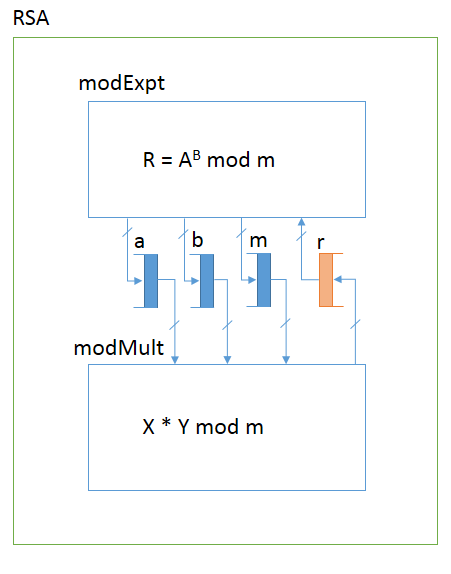
\includegraphics[scale=1]{top_level.png}
    \caption{High level overview. Note that only one of two multipliers is depicted.}
    \label{fig-top}
  \end{centering}
\end{figure}

\subsection{Right to Left Binary Modular Exponentiator}
The modular exponentiator is a circular pipeline (depicted in Figure \ref{fig-expt}).
On each cycle of the pipeline it supplies inputs to the two multipliers.
When the multipliers complete, it stores the results back into the registers.
However one result is discarded if the low bit of {\tt e} is 0.
In fact, our actual implementation will probably not invoke the multiplier
if its result will be discarded anyway.
However, this is simply an optimization, and doesn't hugely affect the overall plan.
On every iteration, the value of {\tt e} is right-shifted by one bit.
When {\tt e} is zero, the loop terminates.

\begin{figure}
  \begin{centering}
    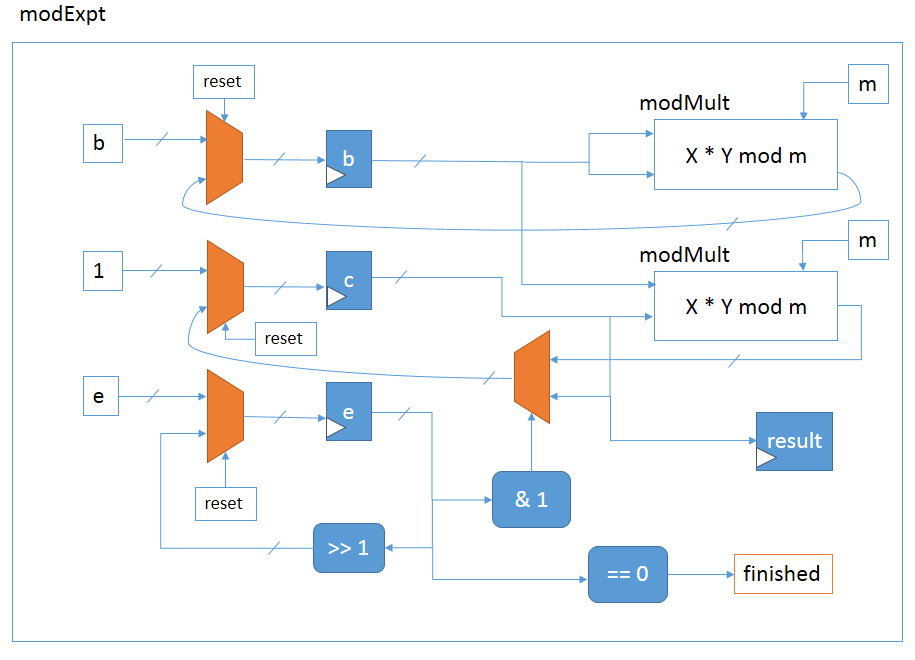
\includegraphics[width=\textwidth]{modexpt.png}
    \caption{Modular exponentiation}
    \label{fig-expt}
  \end{centering}
\end{figure}

\subsection{Interleaved Modular Multiplier}
The interleaved modular has the advantage of not requiring long multiplies, and works with
only left shifts, addition, subtraction, and comparison. Unfortunately, a step of the 
algorithm requires comparing the entire length of the data in the worst case. Additionally,
there are 3 possible add/subtract steps at every step of the algorithm. Therefore, the propagation delay
of each step of the algorithm is prohibitive without pipelining. The naive, unpipelined approach did 
meet timing because of the long propagation delay through the adders.

An overview of the module is pictured in Figure \ref{fig-inter}.

\begin{figure}
  \begin{centering}
    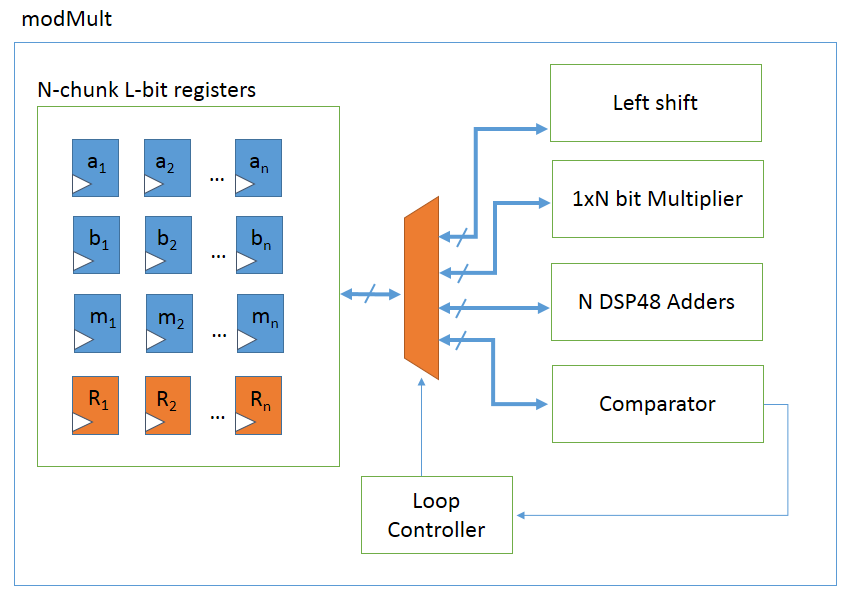
\includegraphics[width=\textwidth]{modmult.png}
    \caption{Interleaved modular multiplication}
    \label{fig-inter}
  \end{centering}
\end{figure}
\section{Implemented Modules}
The modules we implemented are:  {\tt SceMiLayer.bsv, RSAPipeline.bsv, RSA.bsv, ModMultIlvd.bsv, ModExpt.bsv, PipelineAdder.bsv, CLAdder.bsv}

\begin{description}
  \item[SceMiLayer.bsv] We developed two SceMiLayer modules to test different types of designs: one for importing vmh files, and another for importing libgcrypt for simulating our c code.  

  \item[RSAPipelinetypes.bsv] This is the general header file where we define all constant values.  This will make the overall product modular and easy for others to change core elements of design such as number of bits per chunk.
  \item[RSA.bsv]This is a dedicated alternative driver for the RSA module that performs cosimulation with libgcrypt
  \item[ModMultIlvd.bsv] The interleaved modulus multiplier based on the Montgomery Algorithm.  This function computes $a*b$ mod $m$.
  \item[ModExpt.bsv] The modulus exponentiator implements the algorithm described above.  It creates two modulus multiplier to computer $b^e$ mod $m$.
  \item[PipelineAdder, CLAdder.bsv] These modules implement a folded and carry look-ahead adders respectively. 
\end{description}

\subsection{Integer Representation Explorations}
\begin{enumerate}
\item The first interface was a simple {\tt Int\#(1024)} representation. We created a simple adder in order to synthesize our design.
\item The second type of interface is most similar to our C implementation where integers are stored as 64 - 16 bit chunks.
\item The third type of interface uses BRAM to store chunks of the integer throughout the implementation. (This is currently incomplete)
\end{enumerate}
\subsubsection{Difficulties Encountered}
We created a simple adder in order to synthesize our design.  Since we had doubts about the success of this representation this was a vital step before continuing our design. Our concerns were well-founded for the simple {\tt Int\#(1024)} representation: the simple addition of two {\tt Int\#(1024)} were unable to synthesize.
%%%
\chapter*{Implementation Evaluation}
 %What challenges or surprises did you face in implementing your
%design? Did you end up making changes to your original microarchitecture? Did you encounter
%any problems moving the design from simulation to the FPGA?
%Describe the results of your implementation. How many lines of Bluespec code did you have to
%write or modify? What existing IP blocks were you able to make use of in your design (DDR,
%dividers, etc...). What was the device utilization of your design, the clock frequency, and the
%high level throughput (frames per second, bits decoded per second, etc...). Did you meet your
%initial project goals? Why or why not?

\section{Challenges}
Challenges: meeting timing and space constraints on the fpga. We made significant changes to our original microarchitecture to successfully meet our initial project goals.  
 - we fixed timing by modifying the modular multiplication module and space modifying our modular exponentiation architecture.
 
\subsection{Modular Exponentiation}
blbabla write about space constraints and using one multiplier only
include image of modexpt diagram
\subsection{Interleaved Modular Multiplication}
write about using 1 adder and 2 subtraction units. 
To increase the cycle time we do 2 subtractions: p-m and p-2m and select the non negative result at the end.
include diagram
\subsection{Adder Implementation}
Adder was on the critical path
\subsubsection{Clader}
\subsubsection{Multi-cycle Adder}
existing ip blocks used: bram and +
\subsubsection{Syncrhon}
existing ip blocks used



\section{Final Design Results: Space, Timing, and Throughput}
What was the device utilization of your design, the clock frequency, and the
high level throughput (frames per second, bits decoded per second, etc...). Did you meet your
initial project goals? Why or why not?

%%%

%%%
\chapter*{Design Exploration}
 Now that you have a working system, what trade-offs would you be interested
in exploring?
If you didn’t meet your performance targets, why? What are the limiting components in
your design? A detailed analysis of the cycle latency and throughput of each component in
your design may be appropriate. 


\end{document}
